\begin{figure}[H]
\centering
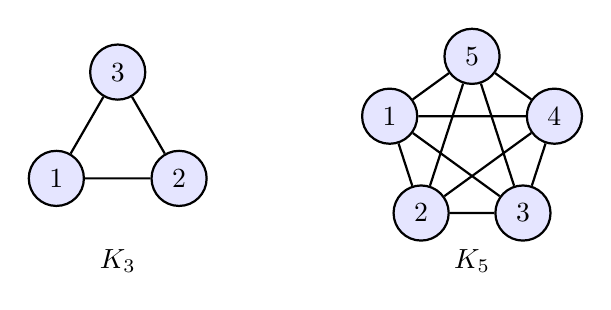
\begin{tikzpicture}[
  vnode/.style={circle, draw, minimum size=7mm, inner sep=0pt, fill=blue!10},
  thick
]
  \begin{scope}[shift={(0,0)}]
    \foreach \i in {1,2,3} {
      \node[vnode] (u\i) at ({90 + \i*360/3}:0.9) {\i};
    }
    \draw (u1) -- (u2) -- (u3) -- (u1);
    \node at (0, -1.5) {$K_3$};
  \end{scope}
  
  \begin{scope}[shift={(4.5,0)}]
    \foreach \i in {1,2,3,4,5} {
      \node[vnode] (w\i) at ({90 + \i*360/5}:1.1) {\i};
    }
    \draw (w1) -- (w2) -- (w3) -- (w4) -- (w5) -- (w1);
    \draw (w1) -- (w3) -- (w5) -- (w2) -- (w4) -- (w1);
    \node at (0, -1.5) {$K_5$};
  \end{scope}
\end{tikzpicture}
\caption{Úplné grafy $K_3$ (3 vrcholy, 3 hrany) a $K_5$ (5 vrcholů, 10 hran).}
\end{figure}